\chapter{Montaje Filastruder}
\label{ane:filastruder}

La filastruder va a ir instalada sobre una plancha de madera en la que también se cablean los elementos usados en el proyecto:

   	\begin{figure}[H]
            \centering
            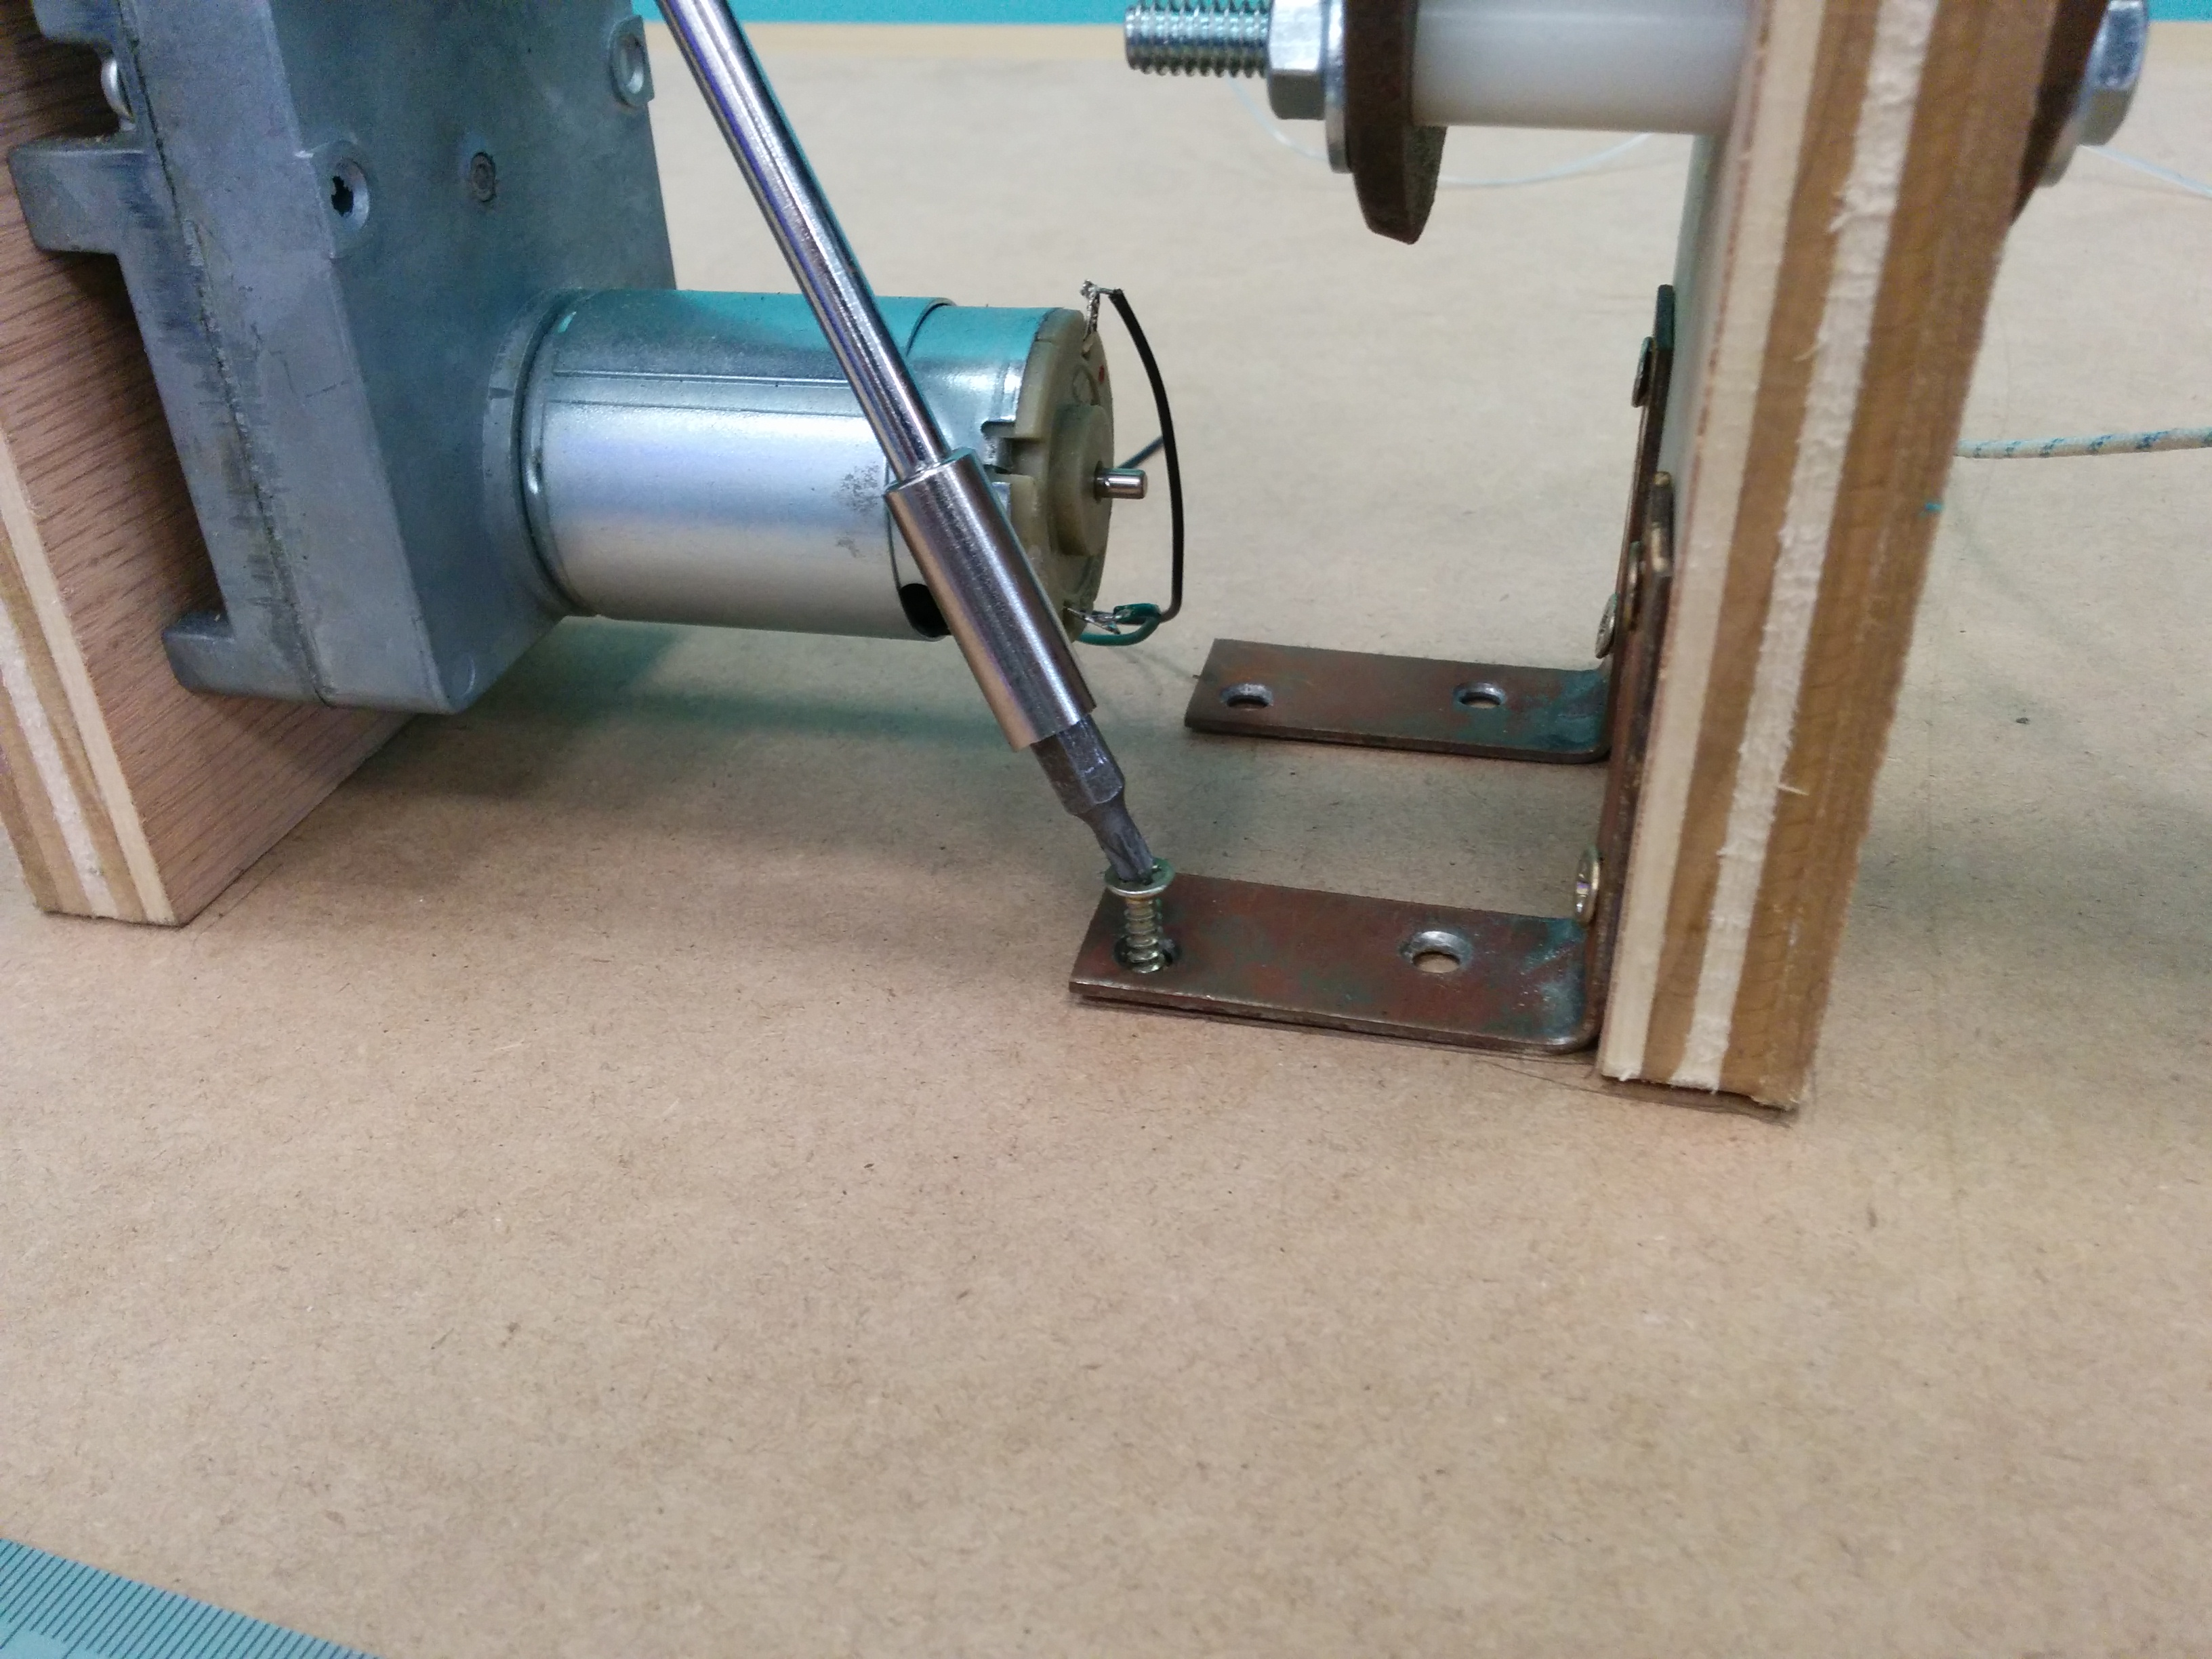
\includegraphics[width=0.6\textwidth]{images/filaextruder/IMG_20150313_114401.jpg}
            \caption{Se ancla la extructura a la base}
            \label{fig:fila_montaje1}
    \end{figure}
    \begin{figure}[H]
            \centering
            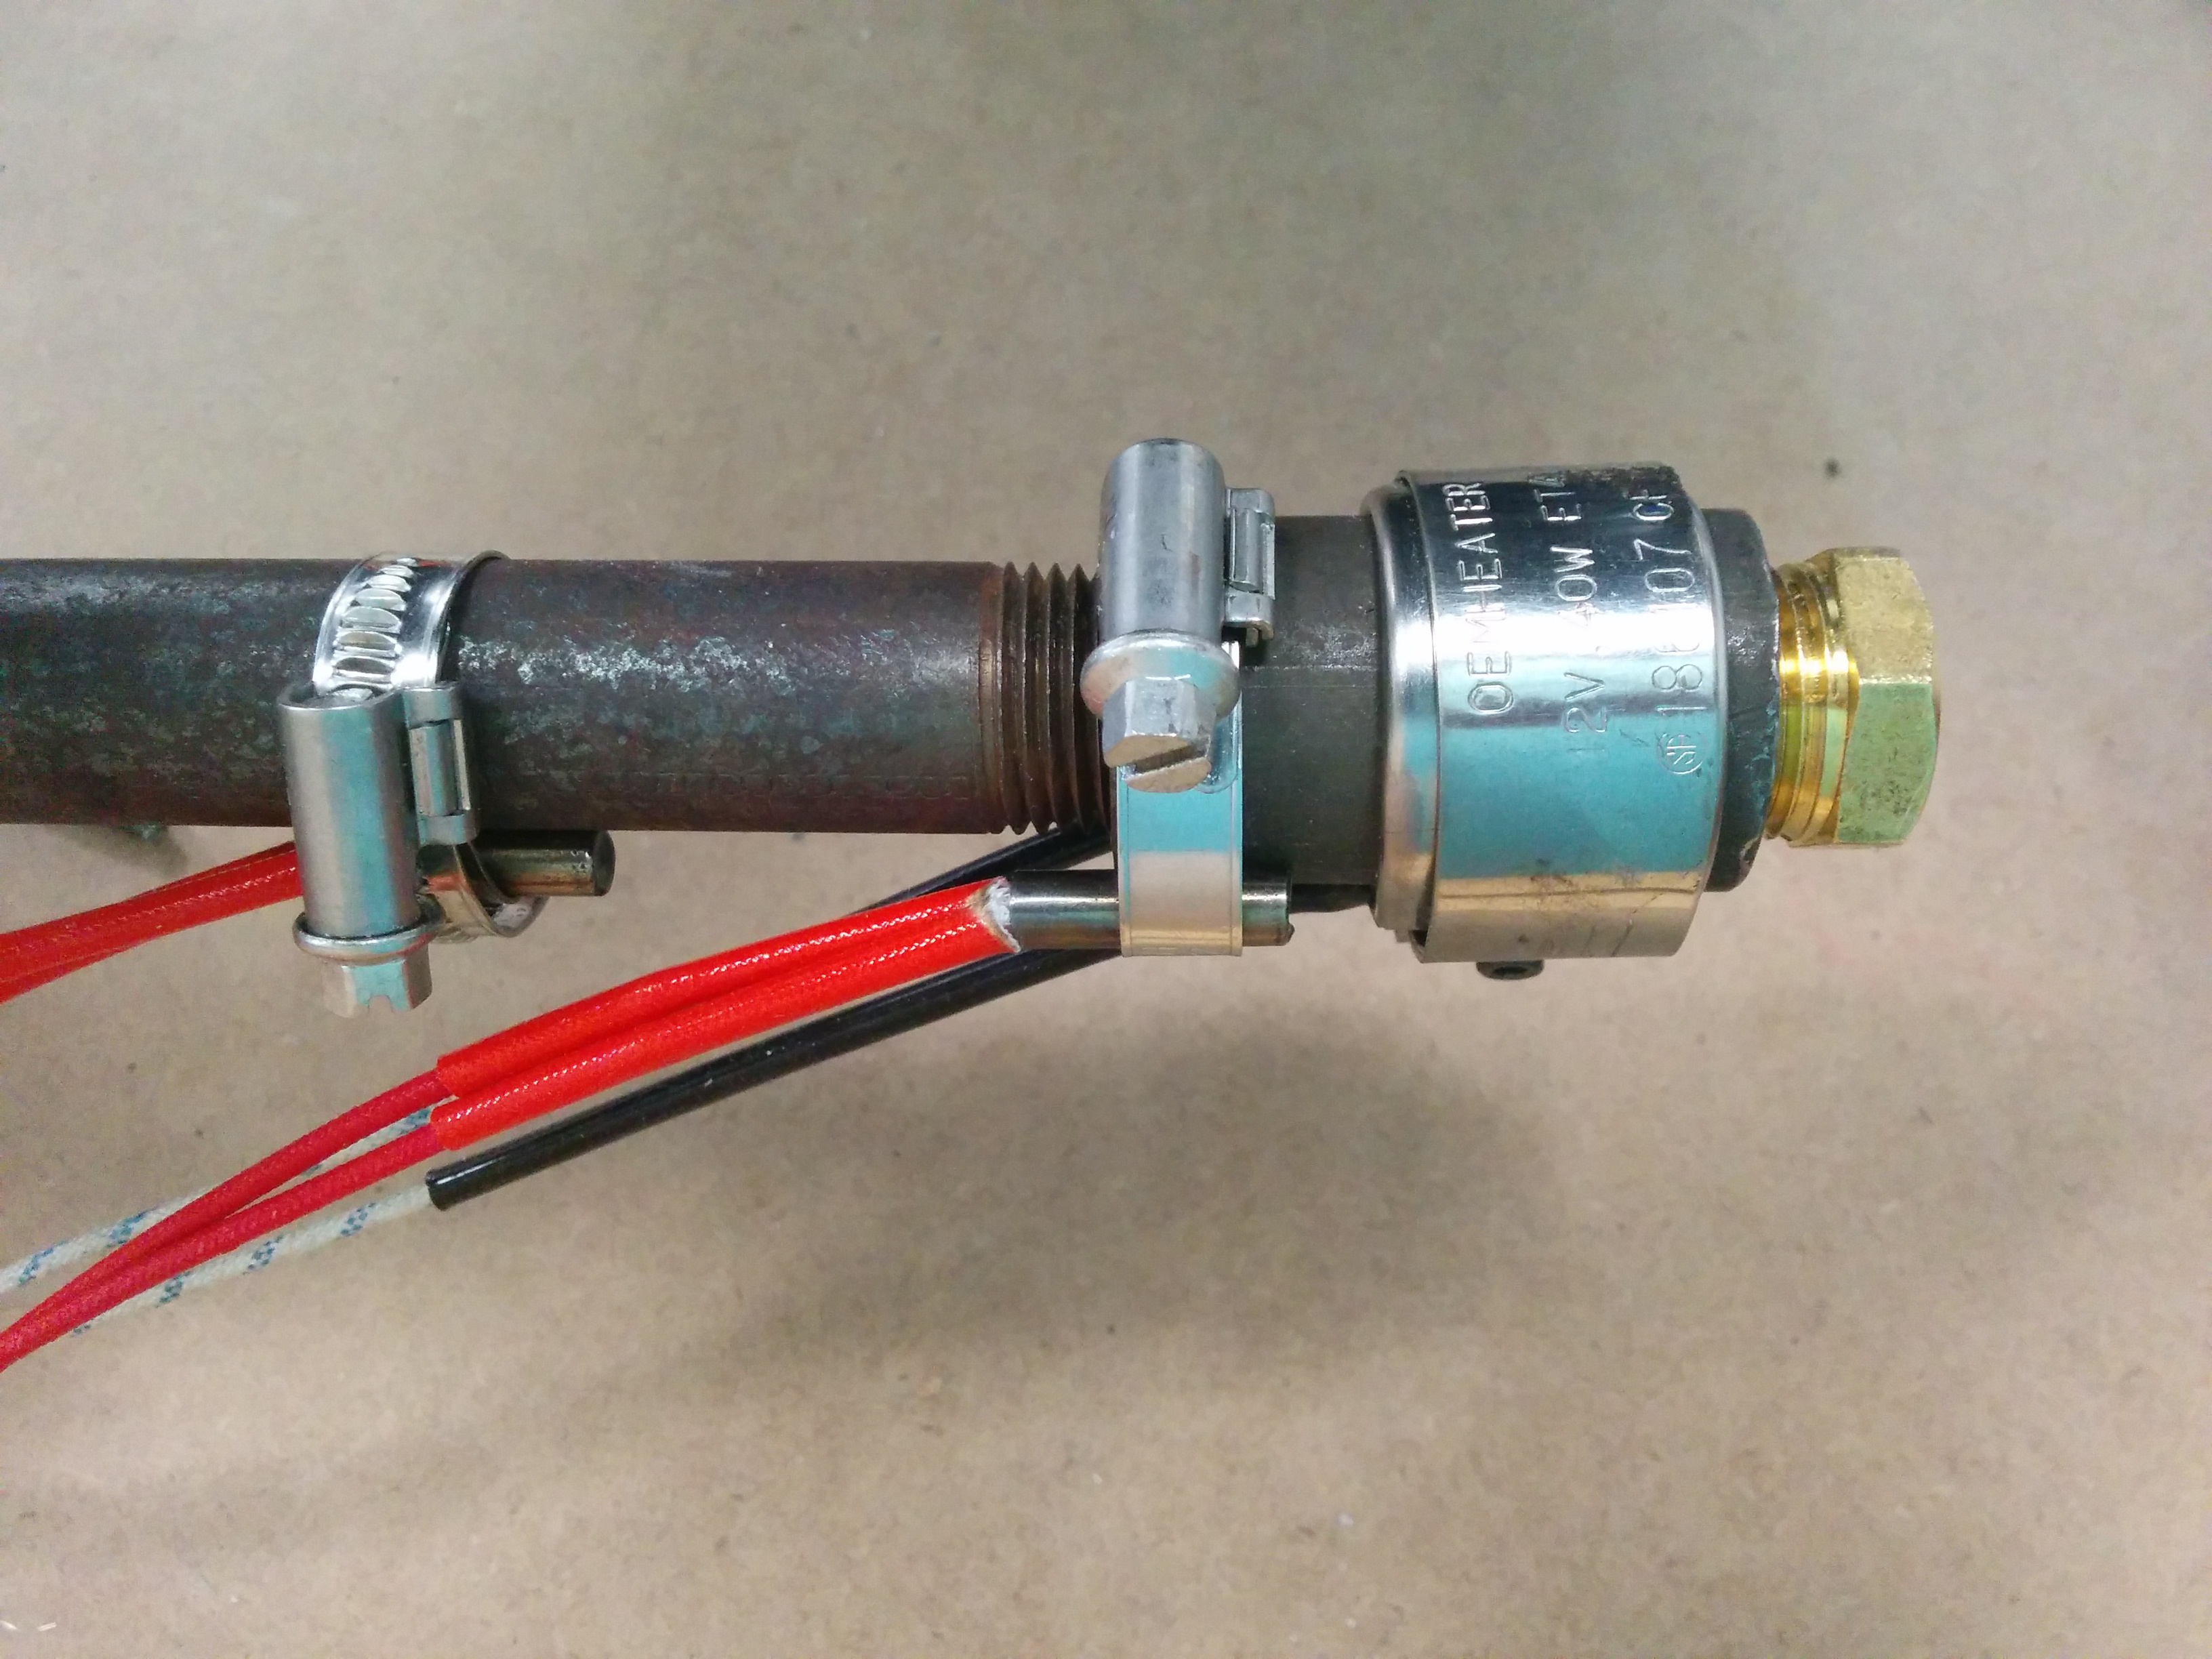
\includegraphics[width=0.6\textwidth]{images/filaextruder/IMG_20150324_175818.jpg}
            \caption{Calefactor en la alimentación y cañon}
            \label{fig:fila_montaje2}
    \end{figure}
    \begin{figure}[H]
            \centering
            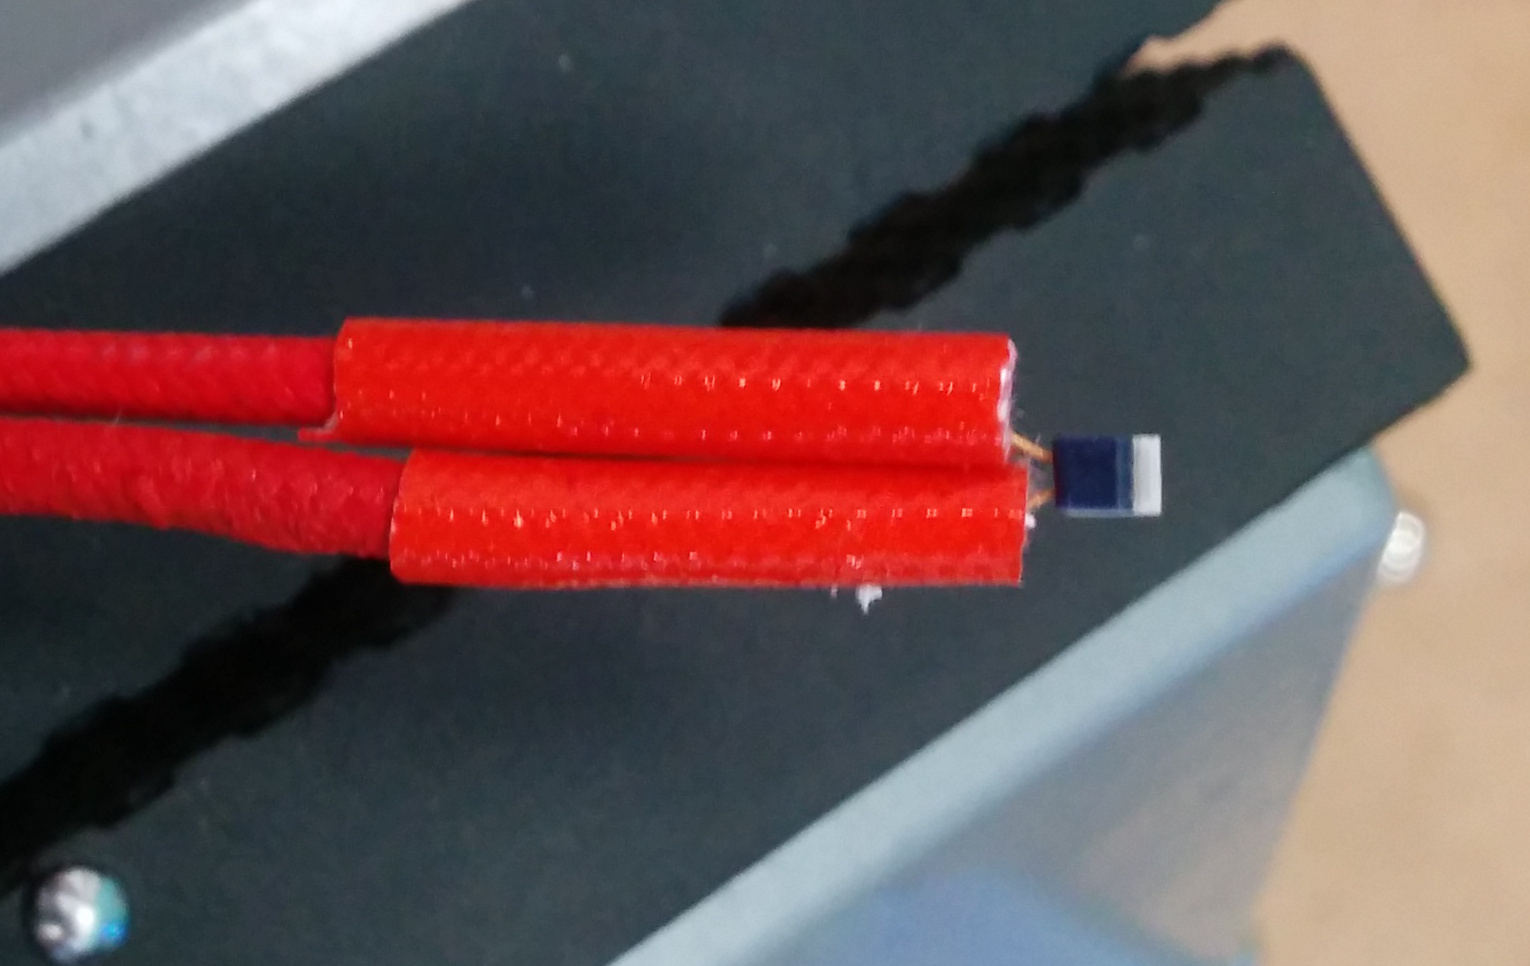
\includegraphics[width=0.6\textwidth]{images/filaextruder/IMG_20150325_145634.jpg}
            \caption{Sensor PT100 de temperatura}
            \label{fig:fila_montaje3}
    \end{figure}

Una vez instalados los cartuchos y las sondas de temperatura en la filastruder, se pasa a aislar el cañón para que la disipación de calor al exterior no sea elevada y poder mantener una temperatura constante.

    \begin{figure}[H]
            \centering
            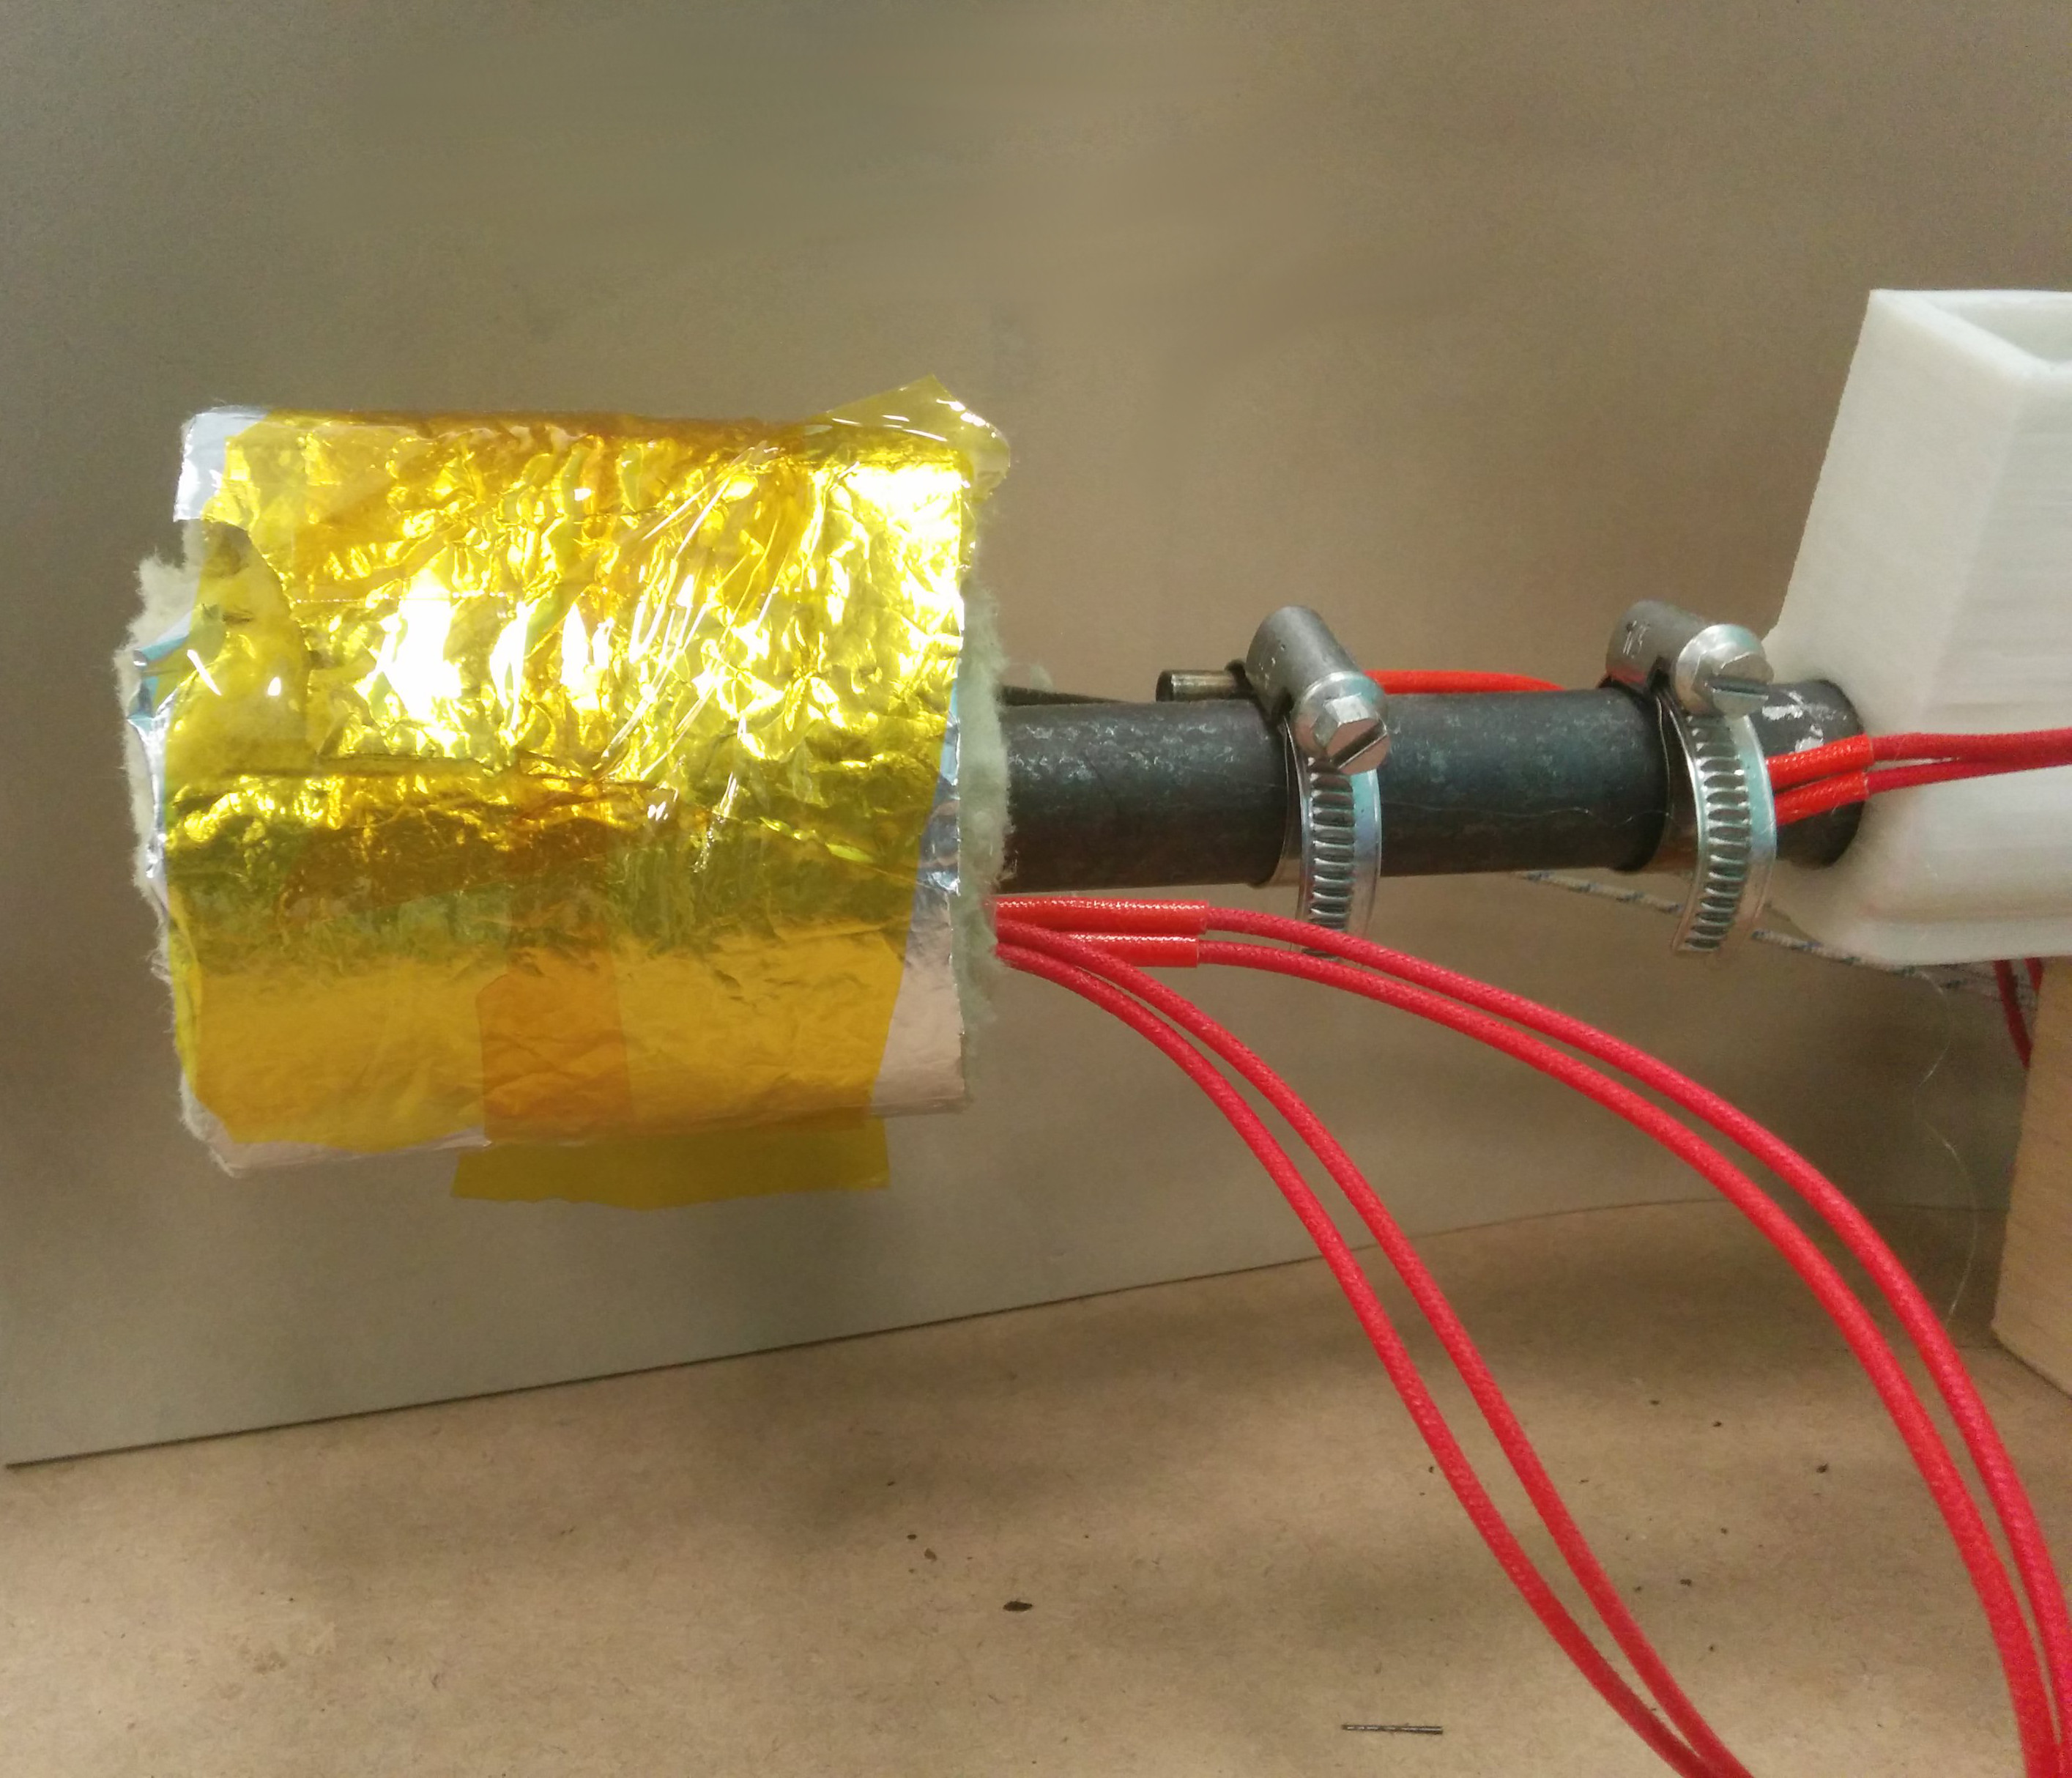
\includegraphics[width=0.4\textwidth]{images/filaextruder/IMG_20150814_132929.jpg}
            \caption{Filastruder montado}
            \label{fig:fila_montaje4}
    \end{figure}

El siguiente paso es cablear todas las señales a un armario que instalaremos en la propia maqueta en el espacio reservado para ello, este armario estará conectado al armario del PLC para poder realizar el control de la maqueta:

    \begin{itemize}
    	\item Sondas de temperatura.
    	\item Reles para controlar las resistencias de potencia y el motor del husillo.
    \end{itemize}

El circuito eléctrico a cablear está indicado en el Anexo \ref{ane:esquemas_electricos}.

    \begin{figure}[H]
            \centering
            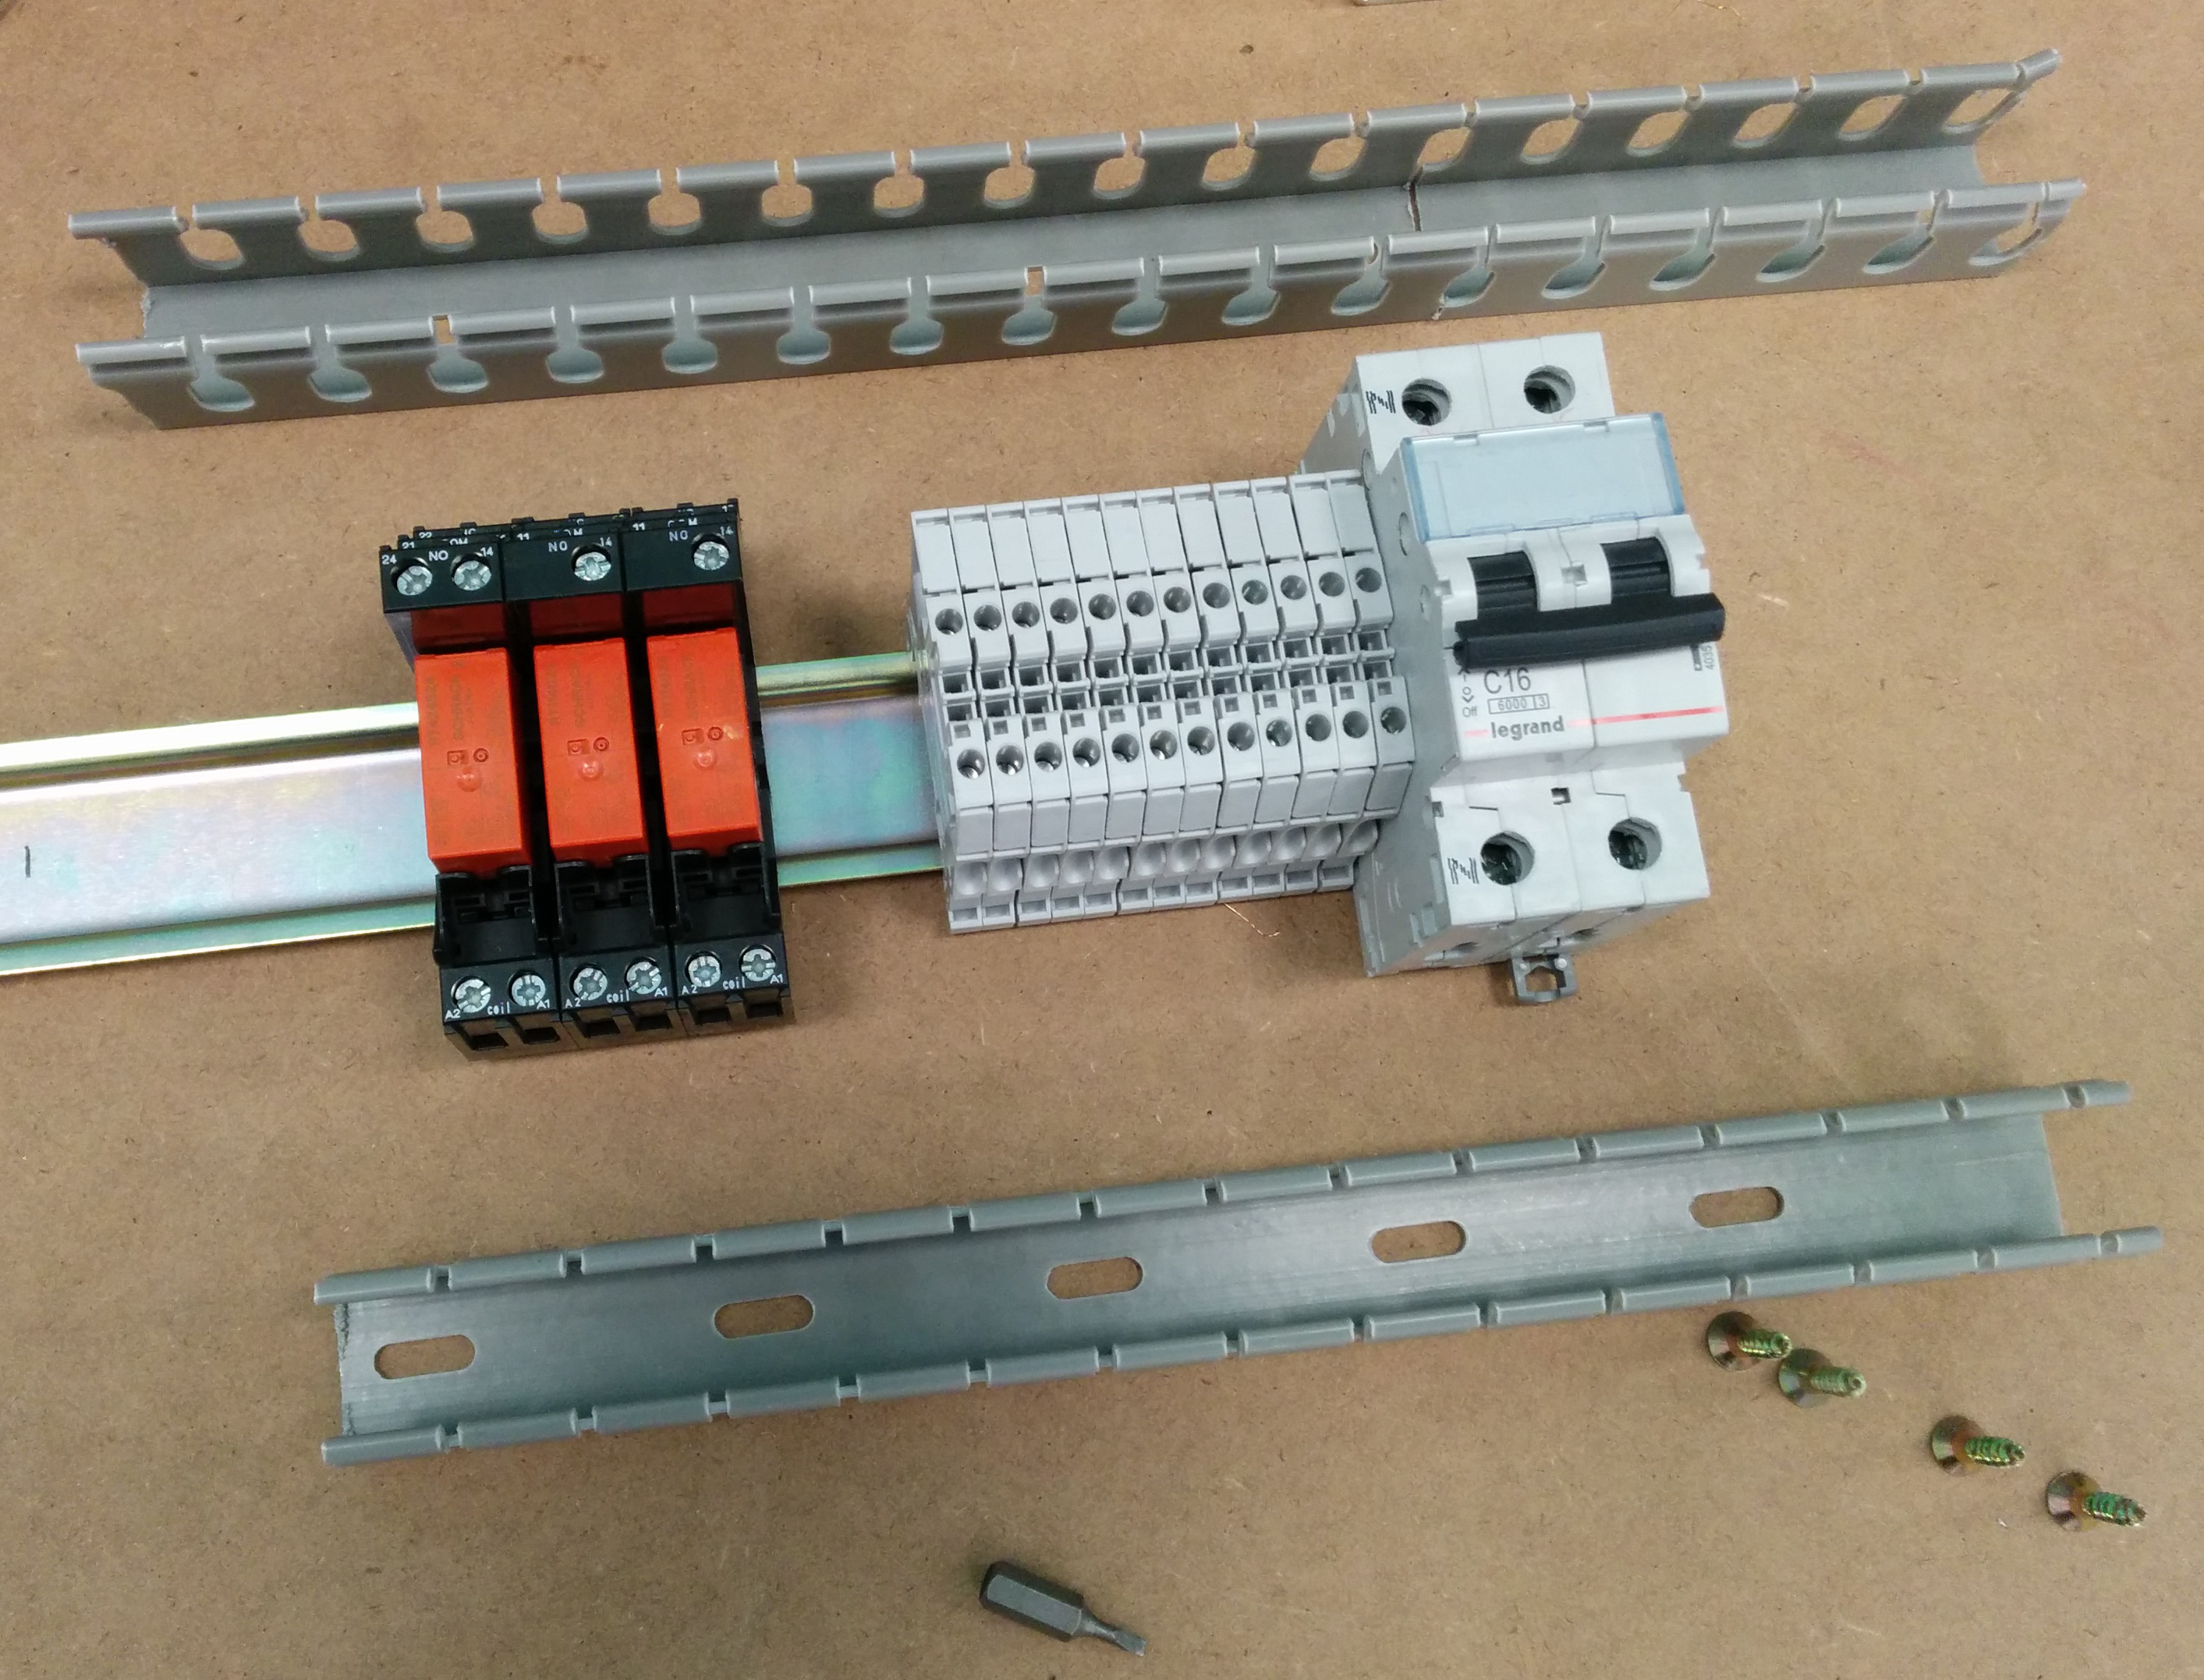
\includegraphics[width=0.5\textwidth]{images/maqueta/IMG_20150324_162200.jpg}
            \caption{Presentación de los componentes en el lugar adecuado.}
            \label{fig:maque_montaje5}
    \end{figure}
    \begin{figure}[H]
            \centering
            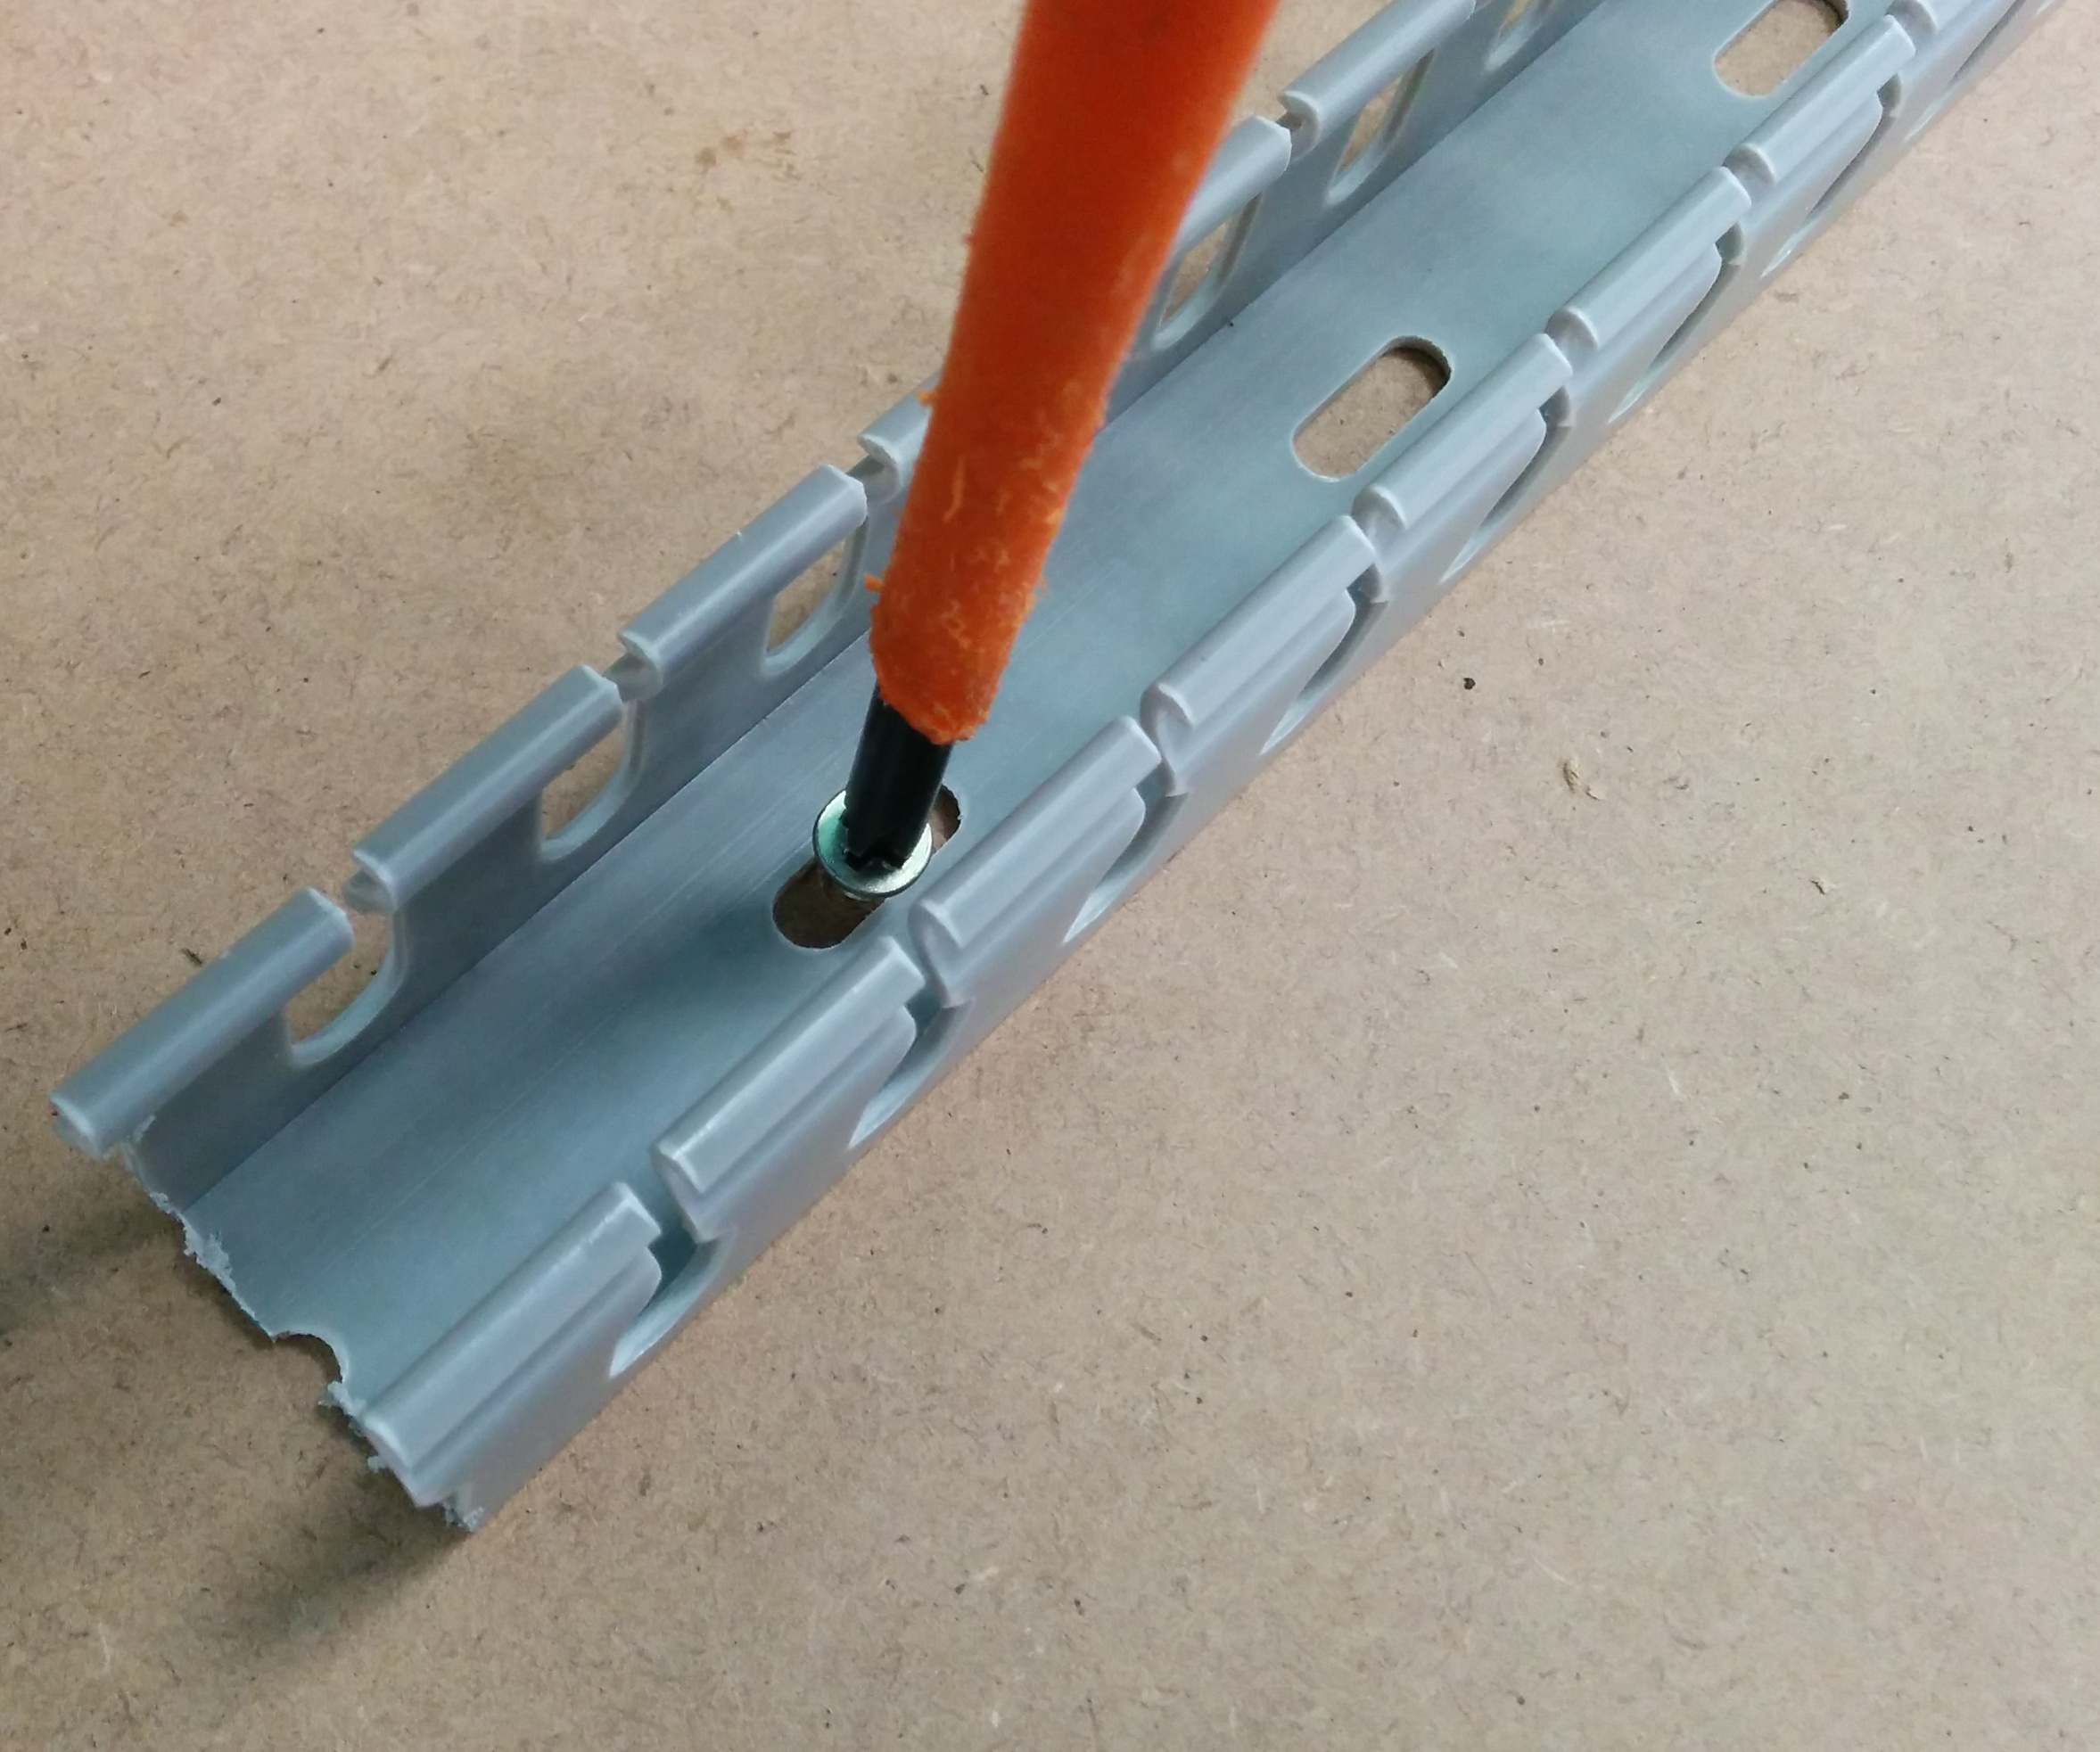
\includegraphics[width=0.5\textwidth]{images/maqueta/IMG_20150324_162705.jpg}
            \caption{Atornillamos las canaletas y guias a la madera.}
            \label{fig:maque_montaje6}
    \end{figure}
    \begin{figure}[H]
            \centering
            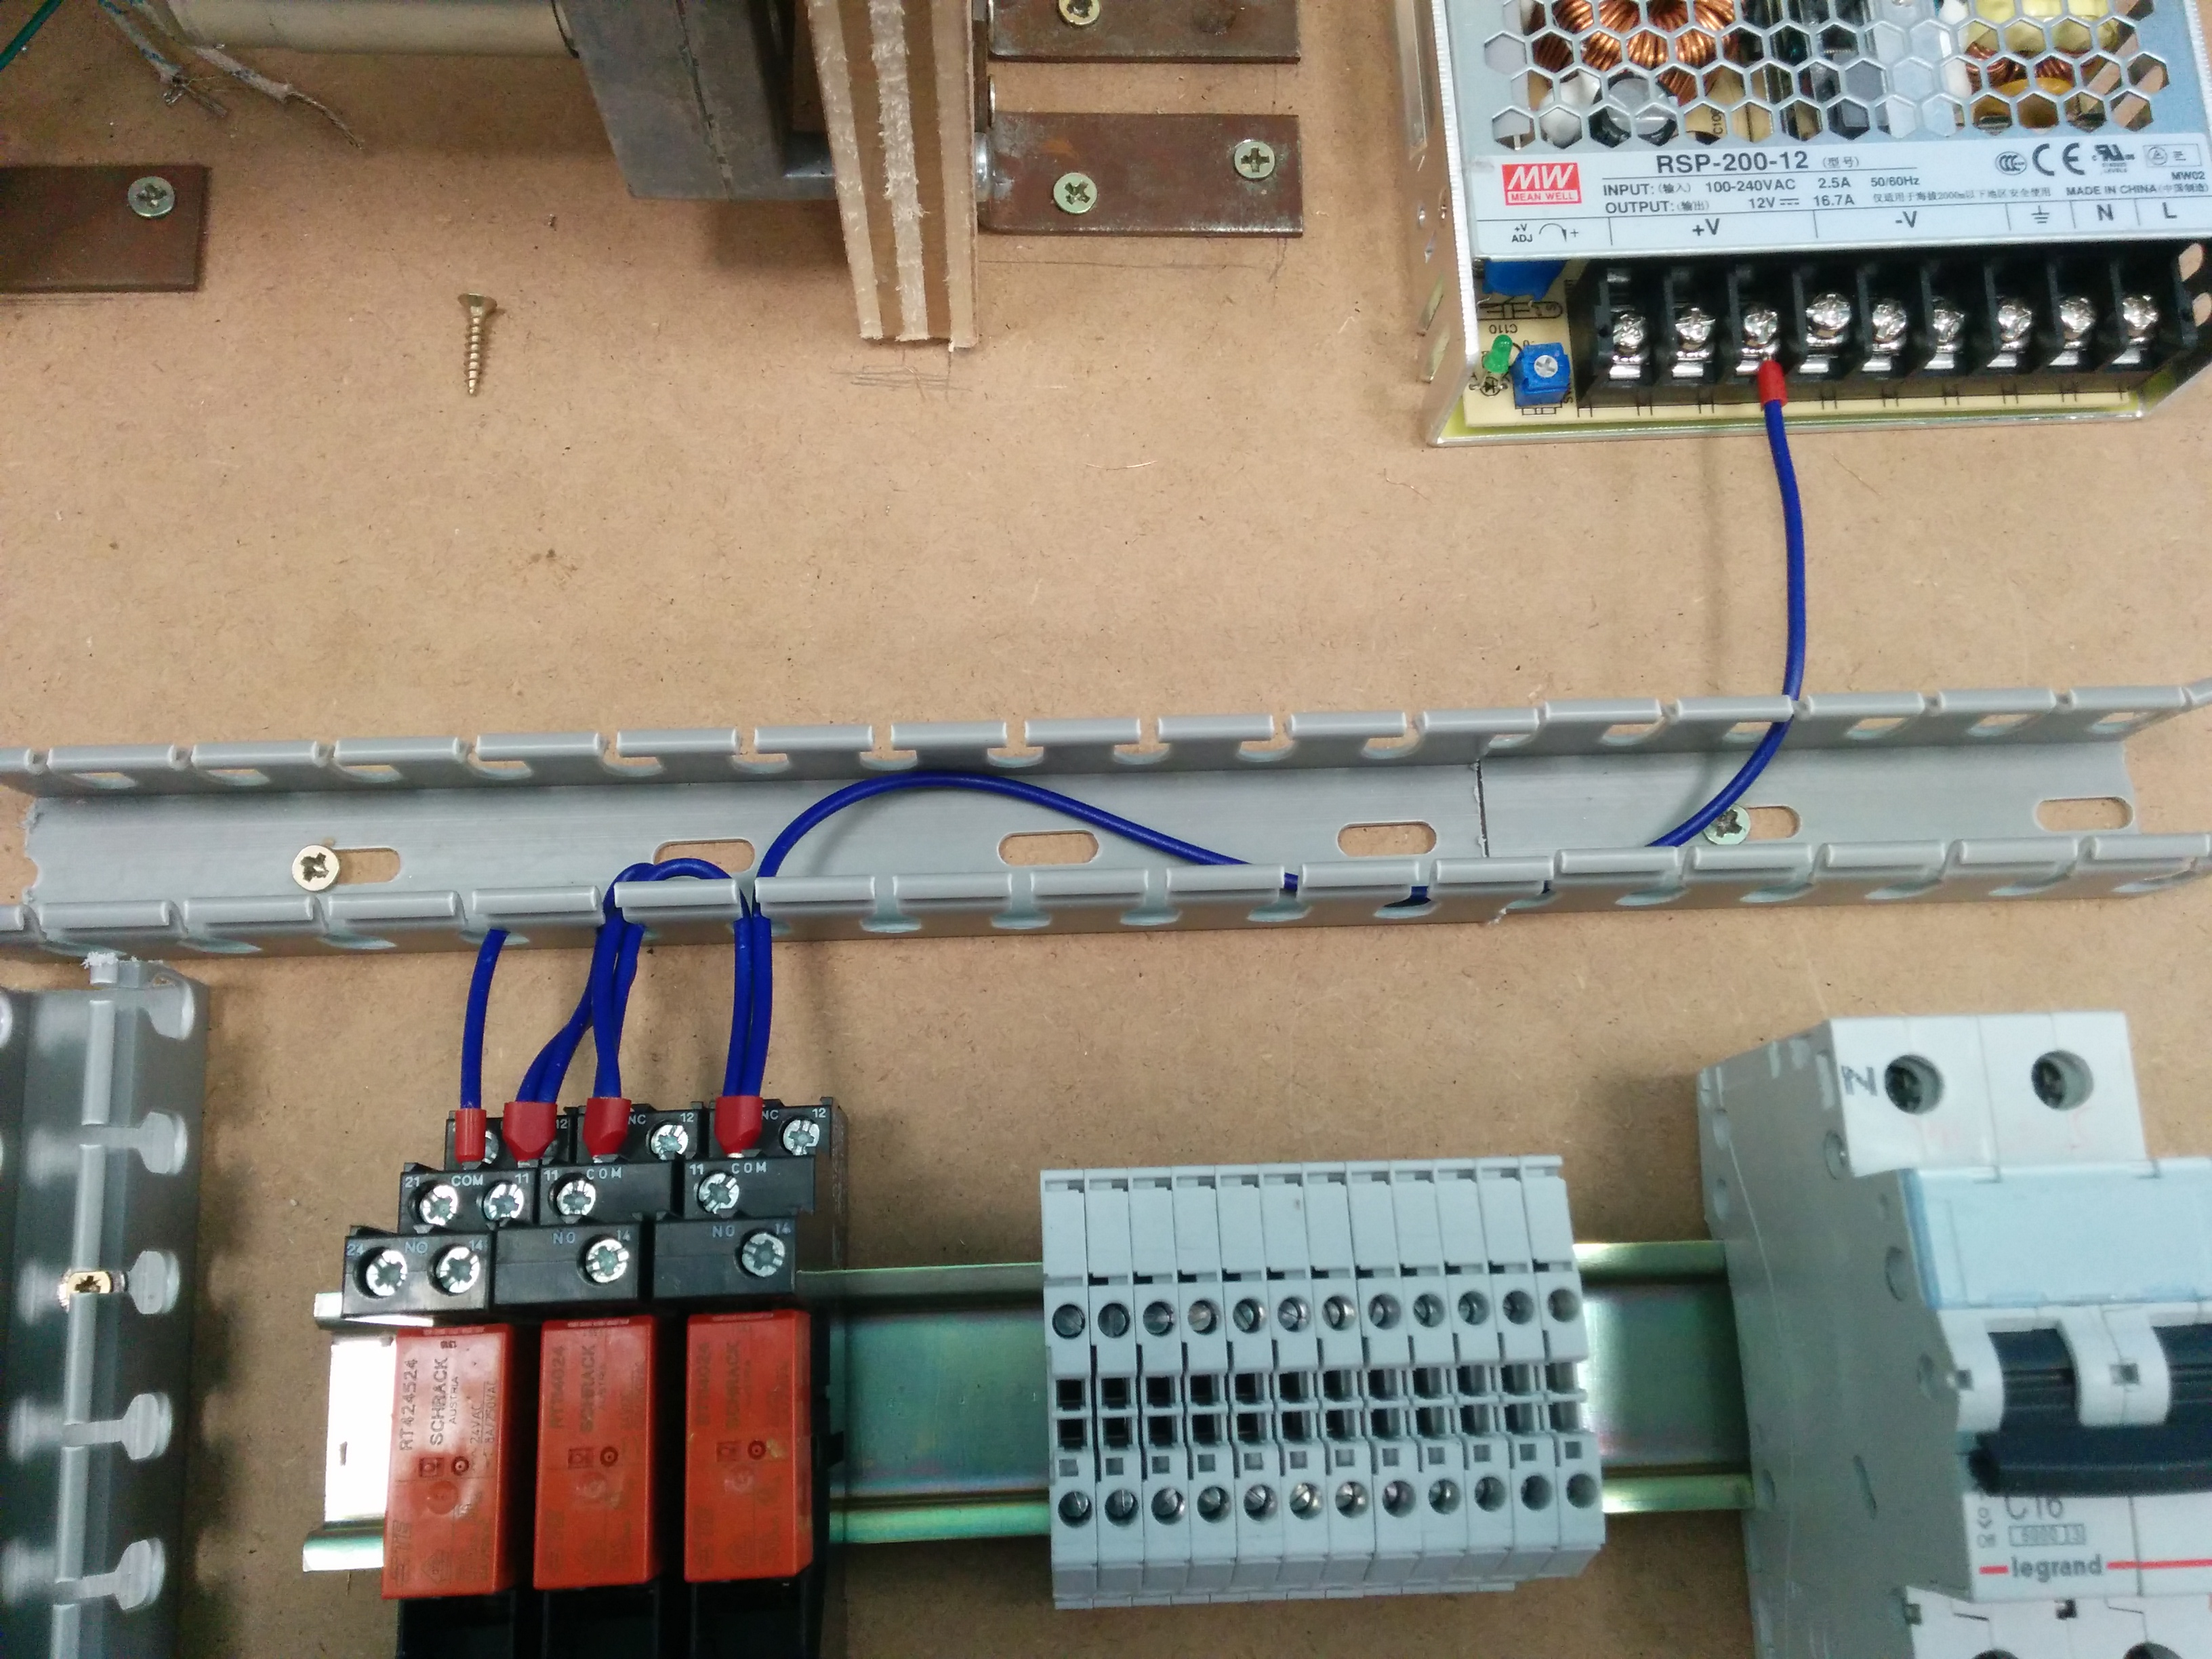
\includegraphics[width=0.5\textwidth]{images/maqueta/IMG_20150324_173716.jpg}
            \caption{Cableamos los componentes según los esquemas.}
            \label{fig:maque_montaje7}
    \end{figure}
    \begin{figure}[H]
            \centering
            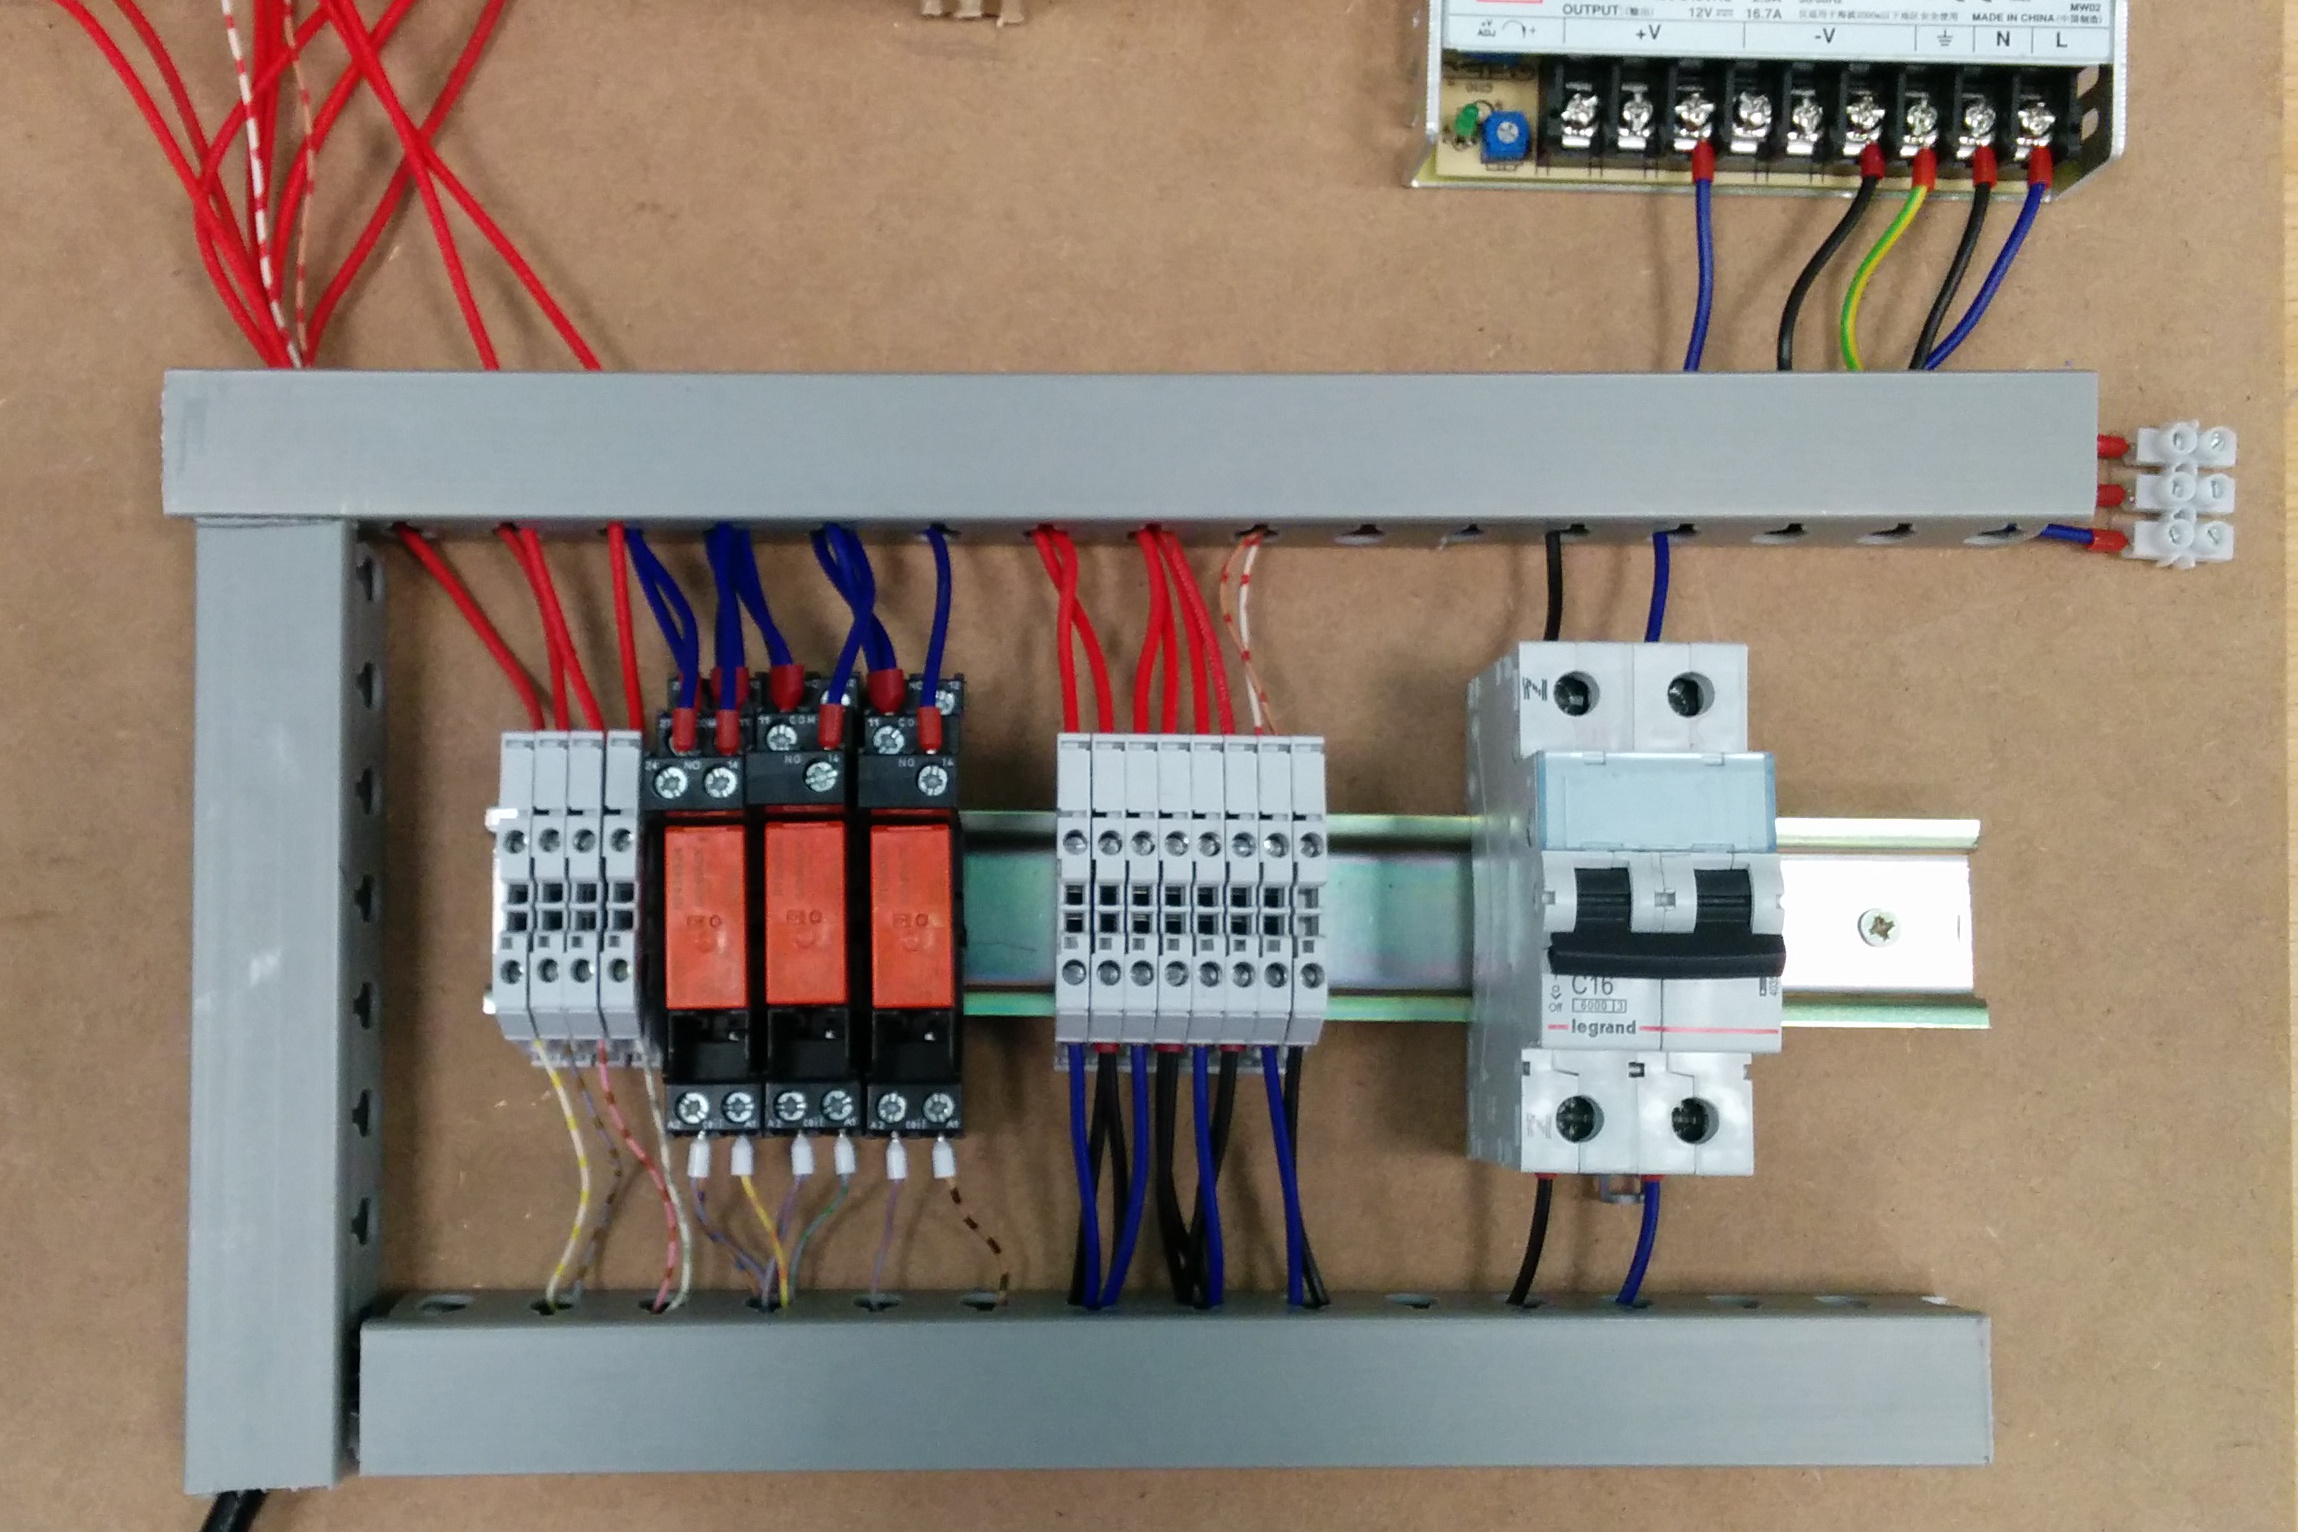
\includegraphics[width=0.5\textwidth]{images/maqueta/IMG_20150331_125243.jpg}
            \caption{Aspecto final cuadro eléctrico maqueta.}
            \label{fig:maque_montaje8}
    \end{figure}